\documentclass{article}

\usepackage{amsmath}
\usepackage{tcolorbox}
\usepackage{verbatim}
\usepackage{hyperref}
\usepackage{fontawesome}
\usepackage{xstring}

\definecolor{codebackground}{rgb}{0.95,0.95,0.95}
\newcommand{\code}[1]{\tcbox[
    on line,
    colback=codebackground, boxsep=2pt,
    colframe=white, boxrule=0pt,
    top=0pt, bottom=0pt, left=0pt, right=0pt
]{\texttt{#1}}}

\hypersetup{
    colorlinks=true,
    linkcolor=black,
    urlcolor=blue
}
\urlstyle{same}
% \linkpy{shared/port} -> \href{file:shared/port.py}{shared.port}
\newcommand{\linkpy}[1]{\href{file:#1.py}{\StrSubstitute{#1}{/}{.}}}

\title{CSCI4230 Project Documentation}
\author{Aidan McHugh, Kai Orita, and Bradley Presier}
\date{April 2023}

\begin{document}
\begin{titlepage}
    \maketitle
    \begin{center}
        \href{https://github.com/2kai2kai2/CSCI4230-project}{GitHub \faGithub} \\
        \vspace*{30em}Note: If links do not work, try opening this file from its directory using Edge or Chrome.
    \end{center}
\end{titlepage}

\tableofcontents

\newpage
\section{Overview}
This project implements a bank ATM system, allowing users to deposit, withdraw, and view their balance through an ATM client.
Due to the lack of a physical machine, no real cash can be exchanged, but we assume for our purposes that this occurs if the ATM client is not an impostor. \\
\\
The implementation operates on three levels with different protocols, which are
\begin{enumerate}
    \item TCP - enabling a connection between client and server
    \item TLS/SSL - authenticating and encrypting communication between client and server
    \item Application - authenticating the user and providing ATM functionality
\end{enumerate}
Note that we consider the server, client, and user as three parties who must each be authenticated at some level.
Also note that the TLS/SSL and Application levels each have their own mode of error handling, which will be discussed in their respective sections.

\section{Usage}
\subsection{Setup}
This project requires Python 3, and has not been tested with versions earlier than Python 3.10.0.
We compile and build local Python packages. This should not be an issue in most Python 3 installations. \\
\\
To install dependencies,
\begin{enumerate}
    \item (optional) Create a virtual environment of your choice.
    \item In this directory, run \code{pip install -r requirements.txt}
\end{enumerate}

\subsection{Run Application}
\begin{enumerate}
    \item Run \code{python server.py} to start the server.
    \item Run \code{python client.py} to start a client instance.
\end{enumerate}

\subsection{Provided Accounts}
\label{sec:ProvidedAccounts}
We have provided several accounts in the database that team blackhat might use or attack:
\subsubsection*{Mallory Malificent}
\textit{This is you!}
\begin{center}
    \begin{tabular}{r|l}
        Card Number     & \code{0000000000000000} \\
        CVC             & \code{666}              \\
        Expiration Date & \code{04/2025}          \\
        PIN             & \code{6969}
    \end{tabular}
\end{center}

\subsubsection*{Charlie Collaborator}
\textit{If you steal from Charlie you're a bad friend. But maybe they'll let you intercept their messages for science.}
\begin{center}
    \begin{tabular}{r|l}
        Card Number     & \code{0000000000000505} \\
        CVC             & \code{111}              \\
        Expiration Date & \code{05/2025}          \\
        PIN             & \code{1111}
    \end{tabular}
\end{center}

\subsubsection*{Alice Allison}
\textit{Alice keeps her bank information very secret.}
\begin{center}
    \begin{tabular}{r|l}
        Card Number     & (random)       \\
        CVC             & (random)       \\
        Expiration Date & \code{05/2025} \\
        PIN             & (random)
    \end{tabular}
\end{center}

\subsubsection*{Bobby McBobface}
\textit{Bobby is less good at keeping secrets than Alice.}
\begin{center}
    \begin{tabular}{r|l}
        Card Number     & \code{0505050505050505} \\
        CVC             & \code{123}              \\
        Expiration Date & \code{06/2023}          \\
        PIN             & (random)
    \end{tabular}
\end{center}

\subsubsection*{Victor Evilson}
\textit{Maybe you feel bad about stealing from Bobby. Victor is very evil so the only issue with stealing from him is that he might come find you.}
\begin{center}
    \begin{tabular}{r|l}
        Card Number     & \code{4111111111111111} \\
        CVC             & (random)                \\
        Expiration Date & \code{09/2026}          \\
        PIN             & (random)
    \end{tabular}
\end{center}

\subsubsection*{Billy Bazillionaire}
\textit{Billy has a lot of money. He probably wouldn't miss it if some disappeared, right?}
\begin{center}
    \begin{tabular}{r|l}
        Card Number     & (random)       \\
        CVC             & (random)       \\
        Expiration Date & \code{12/2100} \\
        PIN             & (random)
    \end{tabular}
\end{center}

\subsection{Structure Overview}
This project is implemented using Python 3 and C++.
Specifically, Python is primarily used while an included Python package is implemented using C++. \\
Throughout this project, we have tried to be thorough in
In the following, we will describe the different components:
\subsubsection{Client/Server}
The client (\code{\href{file:client.py}{client.py}}) and server (\code{\href{file:server.py}{server.py}} and \code{\href{file:database.py}{database.py}}) exist in the main directory of this project.
These are the main entrypoints for this project, and neither party should have access to the internal memory of the other process.
\subsubsection{Shared Libraries}
These libraries are contained in \code{./shared/} and are used by both the server and client (but do not share data between the two).
The libraries in this directory are implemented in Python.
\subsubsection{C++ library}
This Python module is implemented using C++ in \code{./lib/} and will be built by \code{pip} when installing dependencies.

\subsection{Order of Operations}
The operation of this system can be categorized into three primary phases, in addition to the establishment of the TCP connection.
\begin{enumerate}
    \item (TCP Layer) TCP connection established \\
          Client: Connection via \code{\href{https://docs.python.org/3/library/socket.html}{socket{\tiny\faExternalLink}}} \\
          Server: Connection via \code{\href{https://docs.python.org/3/library/socketserver.html}{socketserver{\tiny\faExternalLink}}} using \code{\linkpy{server}.Handler}
    \item (TLS Layer) TLS/SSL handshake establishes \code{\href{file:shared/rpi_ssl.py}{shared.rpi\_ssl}.Session} \\ % For some reason this line breaks if I use \linkpy
          Client: Buffer control given to \code{\linkpy{shared/handshake\_handler}.client\_handle\_handshake} \\
          Server: Buffer control given to \code{\linkpy{shared/handshake\_handler}.server\_handle\_handshake}
    \item (App Layer) Authenticate user to associate \code{\linkpy{database}.Account} with session \\
          Client: Get \code{\linkpy{shared/card}.Card} information from user \\
          Server: Verify information in \code{\linkpy{database}}
    \item (App Layer) Accept routine ATM commands \\
          Client: Get command details and send request to server \\
          Server: Respond to command as appropriate
\end{enumerate}

\section{TLS/SSL Implementation} % ================ TLS/SSL LEVEL ================
At this level, we attempt to implement a simplified version of TLS 1.3.
In this, we attempt to implement cryptographic algorithms in a manner that is usage-independent and reusable.

\subsection{Symmetric Encryption}
We implement only AES-256 with Cipher Block Chaining.
This is contained in the C++ library.
This differs from TLS 1.3 in that CBC-mode is not permitted by TLS 1.3, but is otherwise compliant.

\subsection{Hash Functions}
We implement SHA-1, SHA-256, and SHA-384 in \code{\linkpy{shared/rpi\_hash}}.
However, in keeping with TLS 1.3 and best practices, SHA-1 is not considered a valid option for any purpose.

\subsection{Message Authentication Codes (MACs)}
We implement HMAC in \code{\linkpy{shared/rpi\_hash}}.

\subsection{Digital Signatures}
We implement only RSASSA-PSS (Signature Scheme with Appendix; Probabilistic Signature Scheme) in \code{\linkpy{shared/rsassa\_pss}} as specified in RFC 8017.
This is a preferred digital signature scheme by TLS 1.3 and produces a nondeterministic signature that can be used to verify the original message using the RSA public key.
Our implementation can apply any hash function, but we use SHA-256 and SHA-384 in keeping with TLS 1.3 and best practices.
Both \code{rsa\_pss\_rsae} and \code{rsa\_pss\_pss} modes as defined by TLS 1.3 use this algorithm,
\textbf{TODO: DO WE SUPPORT BOTH OR JUST ONE?}

\subsection{TLS Records}
Each message in a TLS/SSL session is contained within a \href{https://en.wikipedia.org/wiki/Transport_Layer_Security#TLS_record}{TLS record{\tiny\faExternalLink}}.
Functions to encode and decode these, along with a \code{Session} class containing negotiated TLS/SSL session information are implemented in \code{\linkpy{shared/rpi\_ssl}}.
A \code{Session} will only exist after the handshake is completed, and thus the encrypted Alert and Application record implementations are included within it.
The \code{Session} can automatically manage encryption, decryption, and verification/creation of MAC.
Essentially, it provides an interface for the Application-level.

\subsection{TLS/SSL Error Handling}
Should a TLS/SSL-related error occur on this level, an \code{SSLError} will the thrown, which should be reported to the other party
via a corresponding TLS Alert record.
As specified by TLS 1.3, error alerts (all alerts except \code{close\_notify} and \code{user\_canceled}) must be considered fatal.

\section{Application-Level Protocol} % ================ APPLICATION LEVEL ================
This is also partially described in \code{\linkpy{shared/protocol}}.
All messages at the application level should be in the body of an SSL/TLS application record.
This means that application level messages are encrypted and authenticated between the client and server (but not necessarily the user).
Note messages sent follow the format of a client request, followed by a server response.
The server should never spontaneously send a message.

\subsection{Application Message Format}
Each application-level message starts with a single header byte describing what application message type it contains.
These types are defined by the enum \code{\linkpy{shared/protocol}.MsgType}.
The rest of the message contains further details:
\subsubsection{\texttt{ACCOUNT\_AUTH} message type}
This message type is used when authenticating the user.
Prior to user authentication being completed, only \code{ACCOUNT\_AUTH} and possibly \code{ERROR} messages should be sent.
If the server responds successful, user authentication is now completed and the session is permanently associated with the provided account. \\
\\
\textbf{Request Format} \\
\begin{tabular}{llll}
    Start         & Length        & Content     &                                           \\\hline
    \texttt{0x00} & \texttt{0x01} & \code{0x00} & (\code{ACCOUNT\_AUTH} header byte)        \\
    \texttt{0x01} & \texttt{0x0c} & Card Data   & (formatted with \code{Card::to\_bytes()})
\end{tabular} \\
\textbf{Response Format} \\
\begin{tabular}{llll}
    Start         & Length        & Content                    &                                            \\\hline
    \texttt{0x00} & \texttt{0x01} & \code{0x00}                & (\code{ACCOUNT\_AUTH} header byte)         \\
    \texttt{0x01} & \texttt{0x01} & \code{0x00} or \code{0x01} & (unsuccessful or successful, respectively)
\end{tabular} \\
or, if attempts have been exceeded, the response is a fatal \code{ATTEMPTS\_EXCEEDED}
\hyperref[sec:ApplicationError]{error message$_\downarrow$} (this can be considered unsuccessful).

\subsubsection{\texttt{BALANCE} message type}
This message type should only be used after the user is authenticated.
It requests the current account balance of the user from the server. \\
\textbf{Request Format} \\
\begin{tabular}{llll}
    Start         & Length        & Content     &                              \\\hline
    \texttt{0x00} & \texttt{0x01} & \code{0x01} & (\code{BALANCE} header byte)
\end{tabular} \\
\textbf{Response Format} \\
\begin{tabular}{llll}
    Start         & Length        & Content                     &                              \\\hline
    \texttt{0x00} & \texttt{0x01} & \code{0x01}                 & (\code{BALANCE} header byte) \\
    \texttt{0x01} & \texttt{0x08} & big-endian unsigned integer & (account balance in cents)
\end{tabular}

\subsubsection{\texttt{DEPOSIT} message type}
This message type should only be used after the user is authenticated.
It requests that an amount be added to the user's balance.
With a valid ATM client, the corresponding amount of cash will have been inserted.
While \code{DEPOSIT} returns its success status in a similar manner to \code{WITHDRAW}, it will rarely if ever be unsuccessful. \\
\textbf{Request Format} \\
\begin{tabular}{llll}
    Start         & Length        & Content                     &                              \\\hline
    \texttt{0x00} & \texttt{0x01} & \code{0x02}                 & (\code{DEPOSIT} header byte) \\
    \texttt{0x01} & \texttt{0x08} & big-endian unsigned integer & (deposit amount in cents)
\end{tabular} \\
\textbf{Response Format} \\
\begin{tabular}{llll}
    Start         & Length        & Content                    &                                            \\\hline
    \texttt{0x00} & \texttt{0x01} & \code{0x02}                & (\code{DEPOSIT} header byte)               \\
    \texttt{0x01} & \texttt{0x01} & \code{0x00} or \code{0x01} & (unsuccessful or successful, respectively)
\end{tabular}

\subsubsection{\texttt{WITHDRAW} message type}
This message type should only be used after the user is authenticated.
It requests that an amount be deducted from the user's balance.
With a valid ATM client, the corresponding amount of cash will be provided if successful. \\
\textbf{Request Format} \\
\begin{tabular}{llll}
    Start         & Length        & Content                     &                               \\\hline
    \texttt{0x00} & \texttt{0x01} & \code{0x03}                 & (\code{WITHDRAW} header byte) \\
    \texttt{0x01} & \texttt{0x08} & big-endian unsigned integer & (withdraw amount in cents)
\end{tabular} \\
\textbf{Response Format} \\
\begin{tabular}{llll}
    Start         & Length        & Content                    &                                            \\\hline
    \texttt{0x00} & \texttt{0x01} & \code{0x03}                & (\code{WITHDRAW} header byte)              \\
    \texttt{0x01} & \texttt{0x01} & \code{0x00} or \code{0x01} & (unsuccessful or successful, respectively)
\end{tabular}

\subsubsection{\texttt{ERROR} message type}
\label{sec:ApplicationError}
This message type represents a serious error with a request at the application level.
It should only be sent by the server as a response to a client request.
Error codes are defined by the enum \code{AppError} in \code{\linkpy{shared/protocol}}.
See \hyperref[sec:ApplicationErrorCodes]{the next section$_\downarrow$} for error type details. \\
\textbf{Response Format} \\
\begin{tabular}{llll}
    Start         & Length        & Content     &                                    \\\hline
    \texttt{0x00} & \texttt{0x01} & \code{0xFF} & (\code{ERROR})                     \\
    \texttt{0x01} & \texttt{0x01} & error code  & (from \code{AppError} header byte)
\end{tabular}

\subsection{Application Error Codes}
\label{sec:ApplicationErrorCodes}
Application error codes may be sent by the server in an \code{ERROR}-type application message in response to client requests.
They should not occur or be sent in any other situation.
If a valid response exists for the request's own message type (for example insufficient funds for \code{WITHDRAW}), then that will be used instead.

\subsubsection{\texttt{INVALID\_STAGE} (\texttt{0x00})}
This error code may be sent when a application message is sent at an improper time.
For example, if \code{ACCOUNT\_AUTH} messages are sent after the user is authenticated,
or if any \code{BALANCE}, \code{DEPOSIT}, or \code{WITHDRAW} messages are sent before a user is authenticated.
Additionally, this error code may be sent if a nonexistant message type is received.

\subsubsection{\texttt{BAD\_MESSAGE} (\text{0x01})}
This error code may be sent when the content following a valid error code appears to be improperly formatted.
Note that as an application-level error, this will not occur if SSL/TLS issues arise.

\subsubsection{\texttt{ATTEMPTS\_EXCEEDED} (\text{0x02})}
This error will occur if the session has exceeded its permitted failed user authentication attempts
or if the specified card number has recieved too many recent failed login attempts.
As such, it can only occur in response to an \code{ACCOUNT\_AUTH} request.
This error is always fatal.
For more details, see \hyperref[sec:CardLoginAttemptLimit]{below$_\downarrow$}


\subsection{Credit/Debit Cards}
Implementation for card formats and related details is in \code{\linkpy{shared/card}}.
The \code{Card} class represents the fixed-length fields of a standard credit or debit card: \\
\\
\begin{tabular}{rl}
    \centering
    Card Number & A 16-character numerical string which passes the Luhn test. \\
    CVC         & An integer in the range \texttt{[000,999]}.                 \\
    Month       & An integer in the range \texttt{[1,12]}.                    \\
    Year        & An integer in the range \texttt{[2000,3023]}.               \\
    PIN         & An integer in the range \texttt{[0000,9999]}.               \\
\end{tabular}\\
\\
These can be serialized to and from 12 bytes for transmission. \\
Additionally, a \code{Card::generateRandom()} method is provided which will generate a random valid card, optionally with some set fields.

\subsection{Database}
Implementation for the \code{\linkpy{database}} relies heavily on the above \code{\linkpy{shared.card}.Card} implementation.
Primarily, the database is made up of \code{\linkpy{database}.Account} objects, which store information associated with the account, including the card, balance, and accountholder's name.
Note that the name is not used for verification. \\
The database implemented here is intended to represent an abstraction of a real database, but does not fully implement the features of a typical database.
For example, restarting the server will cause a database reset, as all data is stored exclusively in memory. \\
\\
The database exposes the \code{get\_account()} function to the server (and only the server),
and the server is permitted to modify a returned \code{Account}'s balance.
The client and user may not access the database except through the server.

\subsubsection{Login Attempt Limit}
\label{sec:CardLoginAttemptLimit}
The database implements a limit on recent attempts to login with any card number.
If 5 or more failed attempts have occurred in the past 30 minutes (including any attempts that failed because of this),
the database will throw an \code{AttemptsExceededError} that should be caught by the caller and transmitted to the client. \\
Note that to prevent this being used as a method to find other users' card numbers, login attempts for
unused card numbers will have similar behavior in this regard as login attempts providing invalid verification details.
So just as five attempts with a correct card number but incorrect PIN will cause further attempts with this card number to error,
so too will five attempts with an incorrect card number. This error is fatal.

\subsubsection{Generating Accounts}
A number of accounts are generated when the database is started.
Many of these randomize their card fields.
See \hyperref[sec:ProvidedAccounts]{above$^\uparrow$} for the known account details.

\newpage
\section{Provided Server Instance}
For the convenience of the testing and accessibility, a Ubuntu Server Node running 'Server.py is provided.
\begin{center}
    \begin{tabular}{r|l}
        URL  & \textbf{bank.b-rad.solutions} \\
        Port & \textbf{8000}                 \\
    \end{tabular}
\end{center}
The servers Firewall Will block all traffic accept TCP traffic on application port.

\subsection{Configuring Server Address}
In 'client.py' change the first non-import line 'conn = ... ' to the desired URL or IP address as the first arg. Ensure that 'shared/port.py' is correct

\begin{center}
    \code{conn = socket.create\_connection(("localhost", PORT))}
\end{center}

\newpage
\subsection{Root Directory}
\subsubsection{\code{client.py}}
Main Run time file for the program on client side.
\begin{enumerate}
    \item \code{fetch\_record()}
          Fetches a TLS/SSL record from the socket buffer.
    \item \code{input\_card\_legacy()}
          CLI interface for the client to input card details. Does not require ANSI terminal codes or get-key.
    \item \code{input\_card()}
          CLI interface for the client to input card details.
    \item \code{select\_mode\_legacy()}
          CLI interface for the client to select mode of operation. Does not require ANSI terminal codes or get-key.
    \item \code{select\_mode()}
          CLI interface for the client to select mode of operation
    \item \code{request\_balance()}
          This will retrieve the user's account balance from the bank's servers database and return it to the user.
    \item \code{request\_deposit()}
          This will send a request to the servers database for a deposit.
    \item \code{request\_withdraw()}
          This will send a request to the servers database for a withdraw.

          or invalid account information. It may also update the transaction history for the user's account to reflect the withdrawal.
\end{enumerate}

\subsubsection{\texttt{database.py}}
Family of functions to interact with the data of the bank on the server side.
\begin{enumerate}
    \item \code{balance()}
          This will retrieve the user's account balance and return it to the user.
    \item \code{deposit()}
          This will add the deposit amount to the user's account balance and update the account balance accordingly.
          The function would then return a message indicating the successful deposit and the updated account balance, or an error message if the deposit could not be completed.
    \item \code{withdraw()}
          This will check if the user has sufficient funds in their account to cover the withdrawal amount.
          If the user has enough funds, the function would subtract the withdrawal amount from the user's account balance and update the account balance accordingly.
          The function would then return a message indicating the successful withdrawal and the updated account balance, or an error message if the withdrawal could not be completed due to insufficient funds.
    \item \code{\_add\_account()}
          the function is called with the account number, CCV number, and Exp. Date. If the operation is successful, the function returns a success flag and a message indicating that the account was added to the database. If there is an error, the function returns a failure flag and an appropriate error message
    \item \code{get\_account()}
          Retrieves info on a user account.
\end{enumerate}

\subsubsection{\texttt{generate\_keys.py}}
SSH (Secure Shell) key generation involves creating a public and private key pair that can be used for authentication and encryption in secure communication between two devices.

The key generation process usually involves using a program such as ssh-keygen to create a unique key pair.
The public key can be shared with anyone, while the private key is kept secret and stored on the device that will be used to establish the secure connection.

The key pair is created using a mathematical algorithm, typically either RSA or DSA, which generates a unique set of numbers that are used to encrypt and decrypt messages.

\subsubsection{\texttt{requirements.txt}}
This is a Python requirements.txt file that lists the required Python packages for this program. \\
To install the dependencies listed in a requirements.txt file, run \code{pip install -r requirements.txt}. \\
This must be done before using this project.

\subsubsection{\texttt{server.py}}
Main Run time file for the program the Server side.
\begin{enumerate}
    \item \code{fetch\_record()}
    \item \code{handle\_handshake()}
    \item \code{handle\_account\_auth()}
    \item \code{handle\_routine()}
    \item \code{setup()}
    \item \code{message\_handler()}
    \item \code{handle()}
    \item \code{finish()}
\end{enumerate}

\newpage
\subsection{\texttt{lib} Directory}
PyBind is a C++ library that reduces the boilerplate for expose C++ functions and classes to Python.
We use it here to bind our AES implementation written in C++ to Python.

\subsubsection{\texttt{aes.h}}
This file contains is the primary implementation of AES-256 symmetric cipher functionality.
It excludes all bindings for Python, which are included in \code{cpplib.cpp}.

\subsubsection{\texttt{aes\_constants.h}}
This file contains constants used by AES. \\
\textbf{Round Constants}
\code{\_rcon}: This is a table of round constants used in the key schedule of the AES algorithm.
These are ten round constants, but AES-256 uses seven. \\

\textbf{S-box Constants} \\
\code{\_sbox}: This is a substitution table used in the byte substitution step of the AES algorithm. \\
\code{\_inv\_sbox}: This is the inverse of the S-box and is used in the decryption process of the AES algorithm. \\
We provide the functions \code{BYTE sbox(BYTE input)} and \code{BYTE inv\_sbox(BYTE input)} which provide type conversion functionality. \\
\textbf{Galois Multiplication Tables} \\
AES operates over $GF(2^8)$ modulo the irreducible polynomial $x^8 + x^4 + x^3 + x + 1$. \\
However, AES only has a limited number of constants by which values are multiplied (decimal representation $2$, $3$, $9$, $11$, $13$, $14$).
Thus, we use efficient lookup tables rather than implementing Galois Field multiplication.
These lookup tables are used by the \texttt{mixColumns} step. \\
We provide the \code{BYTE GF\_m(BYTE input, unsigned char c)} function which references the correct table \code{c} and multiples by \code{input}.
\subsubsection{cpplib.cpp}
This file contains the C++ side for creating bindings to Python.
\subsubsection{setup.py}
This file contains boilerplate on the Python side for bindings

\newpage
\subsection{\texttt{my\_secrets} Directory}
A directory called \"my\_secrets\" that stores a public key for a client and a server is a folder on a computer system that contains two files, one for the client's public key and the other for the server's public key.
The directory may be protected by appropriate access controls, to ensure that only authorized users or processes can access the files within it.
The files containing the public keys are used to establish secure communication between the client and server, through methods such as SSL/TLS encryption, SSH connections, or other secure protocols.
The directory must be located in a specific location on the file system.

\newpage
\subsection{\texttt{shared} Directory}
A directory called "shared" that stores helper functions for both a client and a server is a folder on a computer system that contains files with code that can be used by both the client and the server.
These files might include common utility functions, configuration files, or other shared resources that are used by both the client and server applications.
The directory may be organized in a specific way, such as by function or module, to make it easy for developers to find the resources they need.
The shared directory must be located in a specific location on the file system, such as in the root directory of the application, or in a dedicated directory for shared resources.
The directory may also be subject to appropriate access controls, to ensure that only authorized users or processes can access the files within it.
The purpose of the shared directory is to promote code reuse and to make it easier to maintain both the client and server applications by avoiding duplicating code that is common to both.

\subsubsection{\texttt{card.py}}
This file contains implementation for the credit/debit \code{Card} class. See above for details.

\subsubsection{\texttt{handshake\_handler.py}} This Python file contains a class or function that handles handshakes between two entities or systems.
Handshakes are a series of communications that establish a connection or exchange information.
\begin{enumerate}
    \item \code{gen\_hash\_input()}
    \item \code{from\_shared\_secret()}
    \item \code{server\_handle\_handshake()}
    \item \code{client\_handle\_handshake()}
\end{enumerate}

\subsubsection{\texttt{keygen.py}} This Python file contains a function or class that generates cryptographic keys used to encrypt and decrypt data, which is essential for secure communication and data storage.
Diffie-Hellman is a cryptographic algorithm used to establish a shared secret between two parties over an insecure communication channel.
It was invented by Whitfield Diffie and Martin Hellman in 1976 and is widely used today in various protocols such as TLS, SSH, and VPNs.
The main idea behind the Diffie-Hellman algorithm is to use the properties of modular arithmetic to enable two parties to agree on a shared secret without actually exchanging it directly over the insecure channel.
The algorithm involves the following steps:
\begin{center}
    \begin{enumerate}
        \item First, the two parties, Alice and Bob, agree on a large prime number and a primitive root modulo that prime.
        \item These values are publicly known and can be shared over the insecure channel.
        \item Alice chooses a secret number, a, and computes A = $g^a$ mod p, where g is the primitive root and p is the prime number.
        \item She sends A to Bob over the insecure channel.
        \item Bob chooses a secret number, b, and computes B = g\^b mod p. He sends B to Alice over the insecure channel.
        \item Alice computes the shared secret as S = B\^a mod p.
        \item Bob computes the shared secret as S = A\^b mod p.
        \item The shared secret, S, can now be used as a symmetric key for encryption and decryption of messages between Alice and Bob.
    \end{enumerate}

\end{center}

One of the main advantages of the Diffie-Hellman algorithm is that it provides perfect forward secrecy, which means that even if an attacker were to obtain the private keys of Alice or Bob at some later time, they would not be able to decrypt past communications because the shared secret was never transmitted over the insecure channel

\subsubsection{\texttt{paillier.py}} This Python file contains a class or function that implements the Paillier cryptosystem, a public-key cryptosystem used for secure data encryption.
Paillier is a public-key cryptosystem invented by Pascal Paillier in 1999.
It is based on the computational difficulty of the decisional composite residuosity assumption (DCRA) problem, which is closely related to the RSA problem.
The Paillier cryptosystem is considered a partially homomorphic encryption scheme, which means that it supports both additive and multiplicative homomorphic operations on ciphertexts.
The Paillier cryptosystem uses two large prime numbers to generate a public key and a private key.
The encryption process involves raising the plaintext to a randomly generated power modulo the product of two prime numbers, and then multiplying the result by another randomly generated value raised to the product of the prime numbers. The decryption process involves raising the ciphertext to a power modulo the product of the prime numbers and then using a modular inverse to recover the original plaintext.
One of the unique features of the Paillier cryptosystem is its homomorphic properties, which allow for computations to be performed on ciphertexts without decrypting them first.
Specifically, the system supports both additive and multiplicative homomorphic operations, meaning that ciphertexts can be added together or multiplied together and the resulting ciphertext will decrypt to the sum or product of the original plaintexts.

\begin{enumerate}
    \item \textbf{genkeys()} The Paillier cryptosystem uses a public key and a private key, which are generated as follows:

          Public Key Generation:
          \begin{enumerate}
              \item Choose two large prime numbers p and q, such that p and q are of equal length in bits and are kept secret.
                    Compute the product of the two primes, n = p*q, which is used as the modulus for both the public and private keys.
              \item Compute the Carmichael's totient function of n, $\lambda(n) = lcm(p-1, q-1)$, which is used to compute the private key.
              \item Choose a random integer g that is relatively prime to n\^2. This is the generator of the cyclic group of integers modulo n.
              \item Compute the public key (n, g), which is made public.
          \end{enumerate}
          Private Key Generation:
          \begin{enumerate}
              \item Choose a random integer L, such that L is relatively prime to $\lambda(n)$.
              \item Compute the private key $\mu = L^{(-1)} $mod$ \lambda(n)$, where $L^{(-1)}$ is the modular multiplicative inverse of L modulo $\lambda(n)$.
          \end{enumerate}
          Once the public and private keys are generated, they can be used for encryption and decryption operations.
          It is important to note that the security of the Paillier cryptosystem relies on the fact that it is difficult to compute the discrete logarithm of g modulo n\^2, and the decisional composite residuosity assumption is true for n.

    \item  \textbf{encrypt()}
    \item  \textbf{decrypt()}

    \item  \textbf{summation()}
          Adds all the chpiertext in list together
\end{enumerate}

\subsubsection{\texttt{port.py}} This Python file contains a class that manages network ports, which are used to establish connections between two entities or systems over a network.

\subsubsection{\texttt{protocol.py}} This Python file contains a class or function that implements a communication protocol, a set of rules and standards that govern how data is exchanged between two entities or systems.

\subsubsection{\texttt{rpi\_hash.py}} This Python file contains a class or function that implements a hashing algorithm, used to convert data into a fixed-length string of characters.
\begin{enumerate}
    \item \code{SHA1()}:
          SHA-1 (Secure Hash Algorithm 1) is a cryptographic hash function that was developed by the United States National Security Agency (NSA) and published as a federal standard in 1995. SHA-1 generates a fixed-sized output of 160 bits, which is typically represented as a 40-digit hexadecimal number.
          SHA-1 takes an input message of any length and produces a fixed-length output that is unique to that input. This makes SHA-1 useful for verifying the integrity of data, as even a small change in the input message will result in a completely different hash value.
          However, SHA-1 has been found to be vulnerable to collision attacks, where two different input messages can produce the same hash value. As a result, it is no longer considered to be a secure cryptographic hash function and has been deprecated in favor of newer, stronger algorithms such as SHA-256 and SHA-3.
          Despite its weaknesses, SHA-1 is still used in some legacy systems and protocols. However, it is recommended that any new systems and applications use stronger and more secure hash functions.
    \item \code{SHA256()}:
          SHA-256 (Secure Hash Algorithm 256) is a cryptographic hash function that is widely used for data integrity and authentication purposes. It is part of the SHA-2 family of hash functions, which were designed by the National Security Agency (NSA) and published by the National Institute of Standards and Technology (NIST) in 2001.
          Like other cryptographic hash functions, SHA-256 takes an input message of any length and produces a fixed-length output of 256 bits. The output is typically represented as a 64-digit hexadecimal number.
          SHA-256 is a stronger hash function than its predecessor, SHA-1, and is less vulnerable to collision attacks.
          It is also faster and more efficient than some other hash functions, such as SHA-512 and Whirlpool.
          SHA-256 is widely used in many applications, including digital signatures, password storage, and blockchain technology.
          It is also used as a component in other cryptographic protocols, such as Transport Layer Security (TLS) and Secure Sockets Layer (SSL).
          Overall, SHA-256 is considered to be a secure and reliable cryptographic hash function for a wide range of applications.
    \item \code{SHA384()}:
          SHA-384 is a cryptographic hash function that belongs to the SHA-2 family of hash functions, which were designed by the National Security Agency (NSA) and published by the National Institute of Standards and Technology (NIST) in 2001.
          SHA-384 is similar to SHA-256, but produces a longer output of 384 bits.
          It uses the same basic algorithm as SHA-256, but with more rounds of processing and a larger initial hash value.
          Like other hash functions, SHA-384 takes an input message of any length and produces a fixed-length output.
          The output is typically represented as a 96-digit hexadecimal number.
          SHA-384 provides a higher level of security than SHA-256, as it has a larger output size and uses more rounds of processing.
          It is particularly useful in applications where stronger security is required, such as in digital signatures and key derivation.
          However, SHA-384 is also slower and less efficient than SHA-256, due to its longer output size and more complex processing.
          As a result, it may not be suitable for applications where speed and efficiency are important.
          Overall, SHA-384 is a secure and reliable cryptographic hash function that can provide a higher level of security than SHA-256 in certain applications.
          However, it should be used carefully, taking into consideration its slower speed and larger output size.
    \item \code{HMAC()}:
          HMAC (short for \"keyed-hash message authentication code\") is a type of message authentication code (MAC) that involves a cryptographic hash function and a secret key.
          HMAC is designed to verify the authenticity and integrity of a message, ensuring that it has not been altered or tampered with during transmission.
          HMAC works by taking a message and a secret key as input and applying a cryptographic hash function (such as SHA-256 or SHA-512) to them.
          The resulting hash value is then combined with the secret key again and hashed again to produce the final HMAC value.
          HMAC is widely used in various security protocols and applications, including secure email, secure remote access, and secure web browsing.
          It provides a simple and efficient way to verify the authenticity and integrity of messages without requiring a secure channel for communication.
\end{enumerate}


\subsubsection{\texttt{rpi\_ssl.py}}
This Python file contains a class or function that implements the SSL (Secure Sockets Layer) protocol used to establish secure connections between two entities or systems over a network.

\subsubsection{\texttt{rsassa\_pss.py}}
This Python file contains a class or function that implements the RSASSA-PSS digital signature algorithm, used to create and verify digital signatures.
Implemented as specified in \href{https://datatracker.ietf.org/doc/html/rfc8017}{RFC 8017}.
\begin{center}
    \begin{enumerate}
        \item \code{MGF1()} Implements the MGF1 mask generation function specified by RSA's PKCSv1.
        \item \code{EMSA\_PSS\_ENCODE()} Encodes a message using EMSA-PSS, which is used by RSA-PSS.
        \item \code{EMSA\_PSS\_VERIFY()} Verifies a message using EMSA-PSS, which is used by RSA-PSS.
        \item \code{RSA\_PSS\_SIGN()} Creates an RSASSA-PSS signature from a message and key.
        \item \code{RSA\_PSS\_VERIFY()} Verifes an RSASSA-PSS signature from a message and signature.
    \end{enumerate}
\end{center}

\subsubsection{\texttt{tls\_handshake.py}}
This Python file contains a class or function that implements the TLS (Transport Layer Security) protocol handshake process, used to establish secure connections between two entities or systems over a network.

\newpage
\section{The Transport Layer Security (TLS) Protocol Version 1.3}
This project is adapted from TLS 1.3 spec, RFC 8446.
This section will overview the protocol and any changes to implmentation makes to it.
Some direct quotations are used.

\subsection{Handshake Protocol Overview}
The cryptographic parameters used by the secure channel are produced
by the TLS handshake protocol.  This sub-protocol of TLS is used by
the client and server when first communicating with each other.  The
handshake protocol allows peers to negotiate a protocol version,
select cryptographic algorithms, authenticate each other,
and establish shared secret keying material.  Once the handshake is
complete, the peers use the established keys to protect the
application-layer traffic.

A failure of the handshake or other protocol error triggers the
termination of the connection

\subsubsection{Message Flow for Full TLS Handshake}
The handshake can be thought of as having three phases (indicated in the diagram below)
\begin{center}
    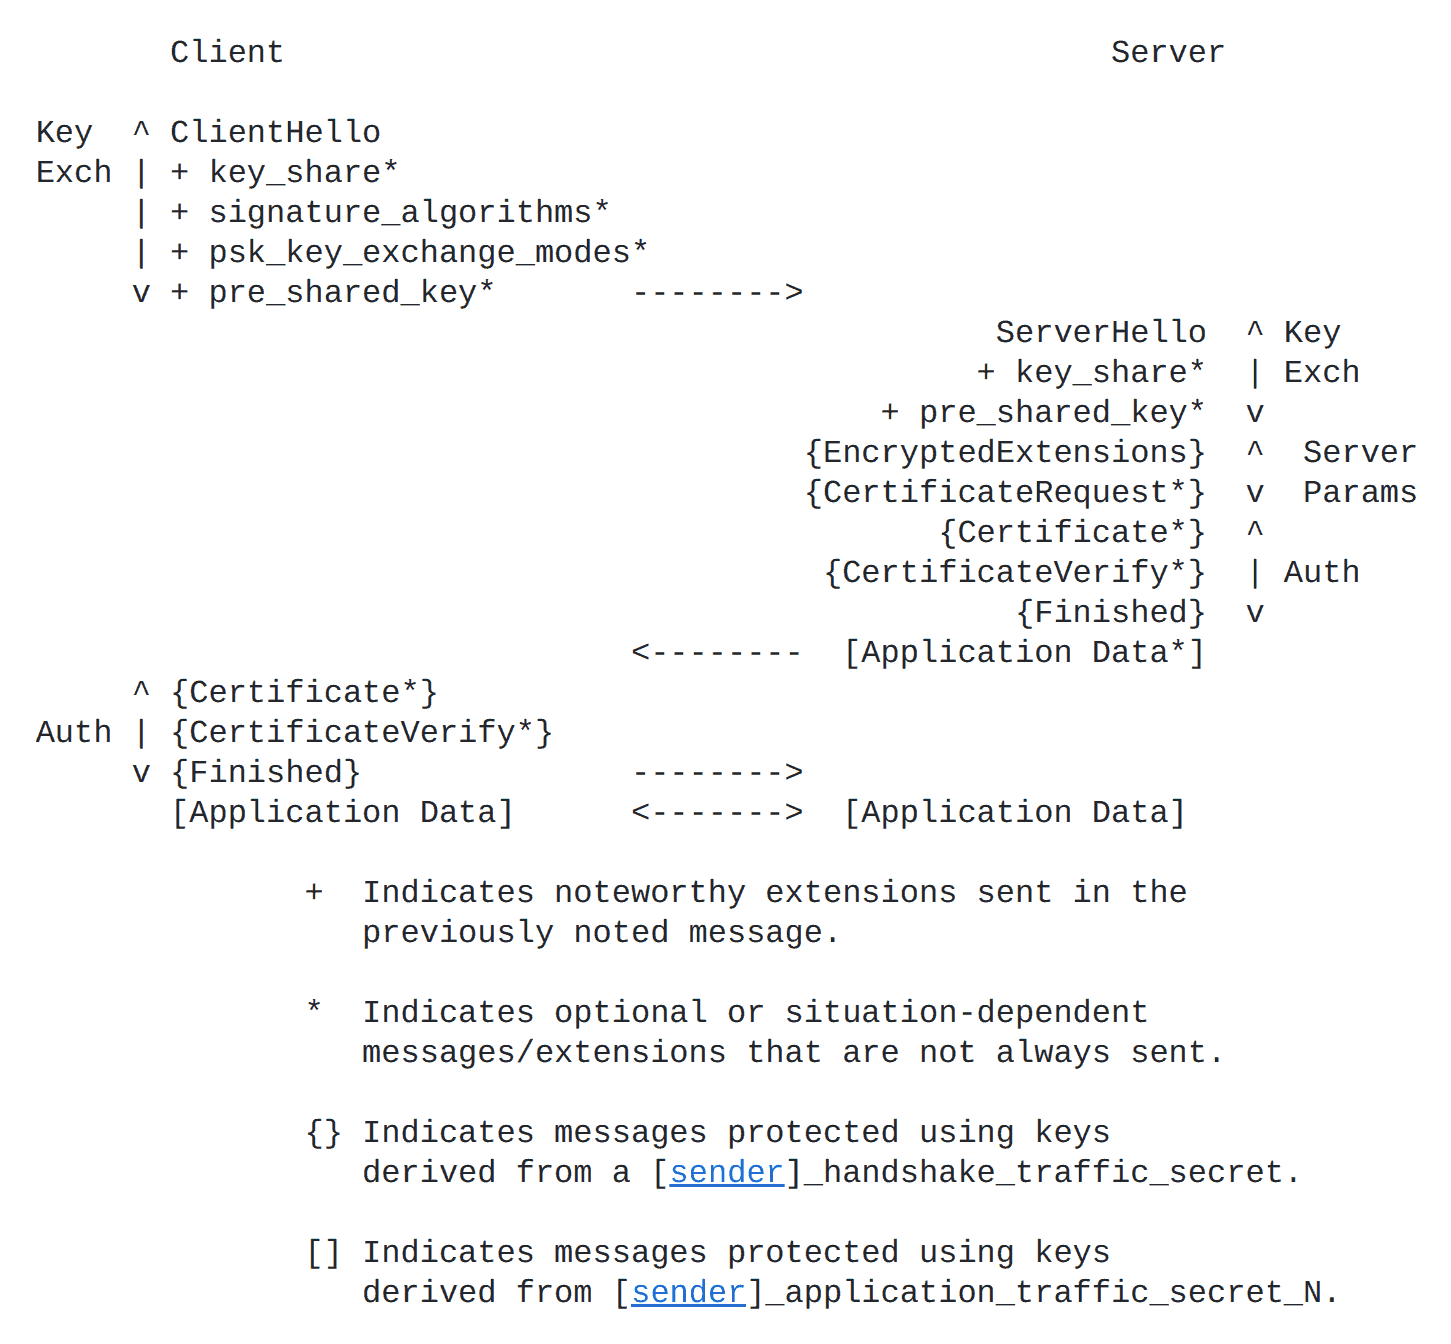
\includegraphics[width=1.1\columnwidth]{media/overview.png}
\end{center}


\begin{enumerate}
    \item Key Exchange: Establish shared keying material and select the
          cryptographic parameters.  Everything after this phase is
          encrypted.
    \item Server Parameters: Establish other handshake parameters
          (whether the client is authenticated, application-layer protocol
          support, etc.).
    \item Authentication: Authenticate the server (and, optionally, the
          client) and provide key confirmation and handshake integrity.
\end{enumerate}


The server then sends two messages to establish the Server
Parameters:
\begin{enumerate}
    \item \textbf{EncryptedExtensions:}  responses to ClientHello extensions that are
          not required to determine the cryptographic parameters, other than
          those that are specific to individual certificates.
    \item \textbf{CertificateRequest:}  if certificate-based client authentication is
          desired, the desired parameters for that certificate. These Params will be deatailed in a later section
\end{enumerate}

Finally, the client and server exchange Authentication messages.  TLS
uses the same set of messages every time that certificate-based
authentication is needed. Specifically:
\begin{enumerate}
    \item \textbf{Certificate:}  The certificate of the endpoint and any per-certificate
          extensions.  This message is omitted by the server if not
          authenticating with a certificate and by the client if the server
          did not send CertificateRequest (thus indicating that the client
          should not authenticate with a certificate).
    \item \textbf{CertificateVerify:}  A signature over the entire handshake using the
          private key corresponding to the public key in the Certificate
          message.  This message is omitted if the endpoint is not
          authenticating via a certificate.
    \item  \textbf{Finished:}  A MAC (Message Authentication Code) over the entire
          handshake.  This message provides key confirmation, binds the
          endpoint's identity to the exchanged keys, and in PSK mode also
          authenticates the handshake.
\end{enumerate}

Upon receiving the server's messages, the client responds with its
Authentication messages, namely Certificate and CertificateVerify (if
requested), and Finished.

At this point, the handshake is complete, and the client and server
derive the keying material required by the record layer to exchange
application-layer data protected through authenticated encryption.
Application Data MUST NOT be sent prior to sending the Finished
message.  Note that while the server may send Application Data prior
to receiving the client's Authentication messages, any data sent
at that point is, of course, being sent to an unauthenticated peer.


\subsection{Handshake Structures}
Messages are stored as a struct that is flattened and reassembled on the other side of the connection. Structs are represented as Python Classes.
\subsubsection{struct ClientHello}
When a client first connects to a server, it is REQUIRED to send the ClientHello as its first TLS message.
Because TLS 1.3 forbids renegotiation, if a server has negotiated
TLS 1.3 and receives a ClientHello at any other time, it MUST
terminate the connection with an \code{unexpected\_message} alert.
After sending the ClientHello message, the client waits for a ServerHello message.

See \href{https://datatracker.ietf.org/doc/html/rfc8446#section-4.1.2}{RFC 8446 section 4.1.2\tiny\faExternalLink} for struct details.

\subsubsection{struct ServerHello}
The server will send this message in response to a ClientHello
message to proceed with the handshake if it is able to negotiate an
acceptable set of handshake parameters based on the ClientHello.

See \href{https://datatracker.ietf.org/doc/html/rfc8446#section-4.1.3}{RFC 8446 section 4.1.3\tiny\faExternalLink} for struct details.

\subsubsection{struct Extensions}
A number of TLS messages contain tag-length-value encoded extensions structures.
\begin{center}
    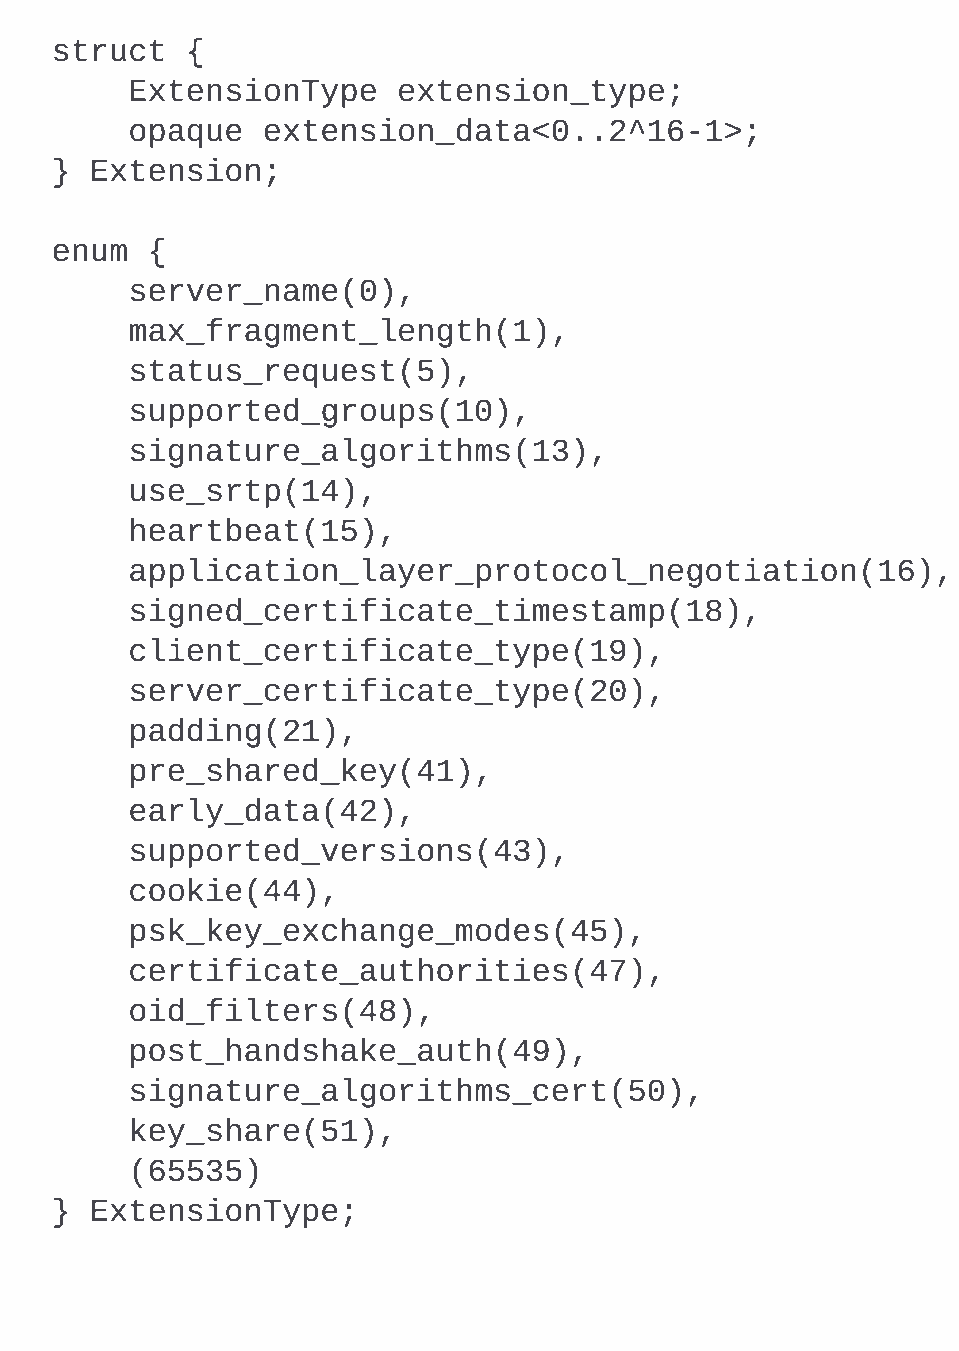
\includegraphics[width=0.8\columnwidth]{media/Extension.png}
\end{center}

Here:
\begin{center}
    \begin{enumerate}
        \item "extension\_type" identifies the particular extension type.
        \item "extension\_data" contains information specific to the particular extension type.
    \end{enumerate}
\end{center}

\subsubsection{struct Finished}
The Finished message is the final message in the Authentication Block.
It is essential for providing authentication of the handshake and of the computed keys.

Recipients of Finished messages MUST verify that the contents are
correct and if incorrect MUST terminate the connection with a \code{decrypt\_error} alert.

Once a side has sent its Finished message and has received and validated the Finished message from its peer,
it may begin to send and receive Application Data over the connection.

See \href{https://datatracker.ietf.org/doc/html/rfc8446#section-4.4.4}{RFC 8446 section 4.4.4\tiny\faExternalLink} for struct details.

\subsection{Transcript Hash}
Many of the cryptographic computations in TLS make use of a
transcript hash.  This value is computed by hashing the concatenation
of each included handshake message, including the handshake message
header carrying the handshake message type and length fields, but not
including record layer headers.  I.e., This is done with SHA256\\

\texttt{Transcript-Hash(M1, M2, ... Mn) = Hash(M1 $||$ M2 $||$ ... $||$ Mn)}

\subsection{Signature Algorithms: RSASSA-PSS}
RSASSA-PSS (RSA Signature Scheme with Appendix - Probabilistic Signature Scheme) is a digital signature scheme that combines the RSA algorithm with probabilistic methods for added security.
RSASSA-PSS is considered to be more secure than the older RSA-PKCS\#1 v1.5 signature scheme,
as it provides protection against certain types of attacks such as chosen-message attacks and key-recovery attacks.
See above for details on included cryptographic primitives.

\subsection{Certificates}
%\subsubsection{Server Certificate Selection}

%\subsubsection{Client Certificate Selection}

\subsubsection{Receiving a Certificate Message}
If the server supplies an empty Certificate message, the client MUST abort the handshake with a decode\_error alert.
While we implement SHA-1, we only permit SHA-256 or SHA-384.

\subsubsection{struct CertificateRequest}
A server which is authenticating with a certificate will request a certificate from the client.
This message, if sent, MUST follow EncryptedExtensions.

See \href{https://datatracker.ietf.org/doc/html/rfc8446#section-4.3.2}{RFC 8446 section 4.3.2\tiny\faExternalLink} for struct details.


\subsubsection{struct CertificateVerify}
This message is used to provide explicit proof that an endpoint possesses the private key corresponding to its certificate.
The CertificateVerify message also provides integrity for the handshake up to this point.
We authenticate via certificate, so both the server and client must send this message.
When sent, this message MUST appear immediately after the Certificate message and immediately prior to the Finished message.

See \href{https://datatracker.ietf.org/doc/html/rfc8446#section-4.4.3}{RFC 8446 section 4.4.3\tiny\faExternalLink} for struct details.


\end{document}